\header{6}
\chapter{Schiemannen}
\section{Inleiding}
In dit hoofdstuk worden de knopen geleerd die belangrijk zijn tijdens het varen. Je moet de knopen kunnen maken en begrijpen wanneer en waarom je ze gebruikt. Onderaan dit hoofdstuk staat een tabel waar je knopen worden afgetekend door een instructeur. 
\section{De knopen}
\subsection{Halve steek \hfill \hspace{2 cm} \textit{Figuur \ref{pic:halve_steek}} } 
Een halve steek leg je wanneer je een touw vast wil leggen waar weinig kracht op komt. De halve steek is de basis voor veel knopen en steken.
\subsection{Slipsteek \hfill \textit{Figuur \ref{pic:slip_steek}}}
De slipsteek kan alleen gebruikt worden in situaties waar weinig kracht op de lijn komt. Het voordeel van een slipsteek is dat hij snel los te maken is.
\subsection{Achtknoop \hfill \textit{Figuur \ref{pic:achtknoop}}}
Een achtknoop wordt gebruikt om een verdikking in een touw te maken. Hiermee voorkom je bijvoorbeeld dat een touw door een blok schiet. 
\begin{figure}[h]
  \centering
  \begin{minipage}[b]{0.32\textwidth}
  \centering
    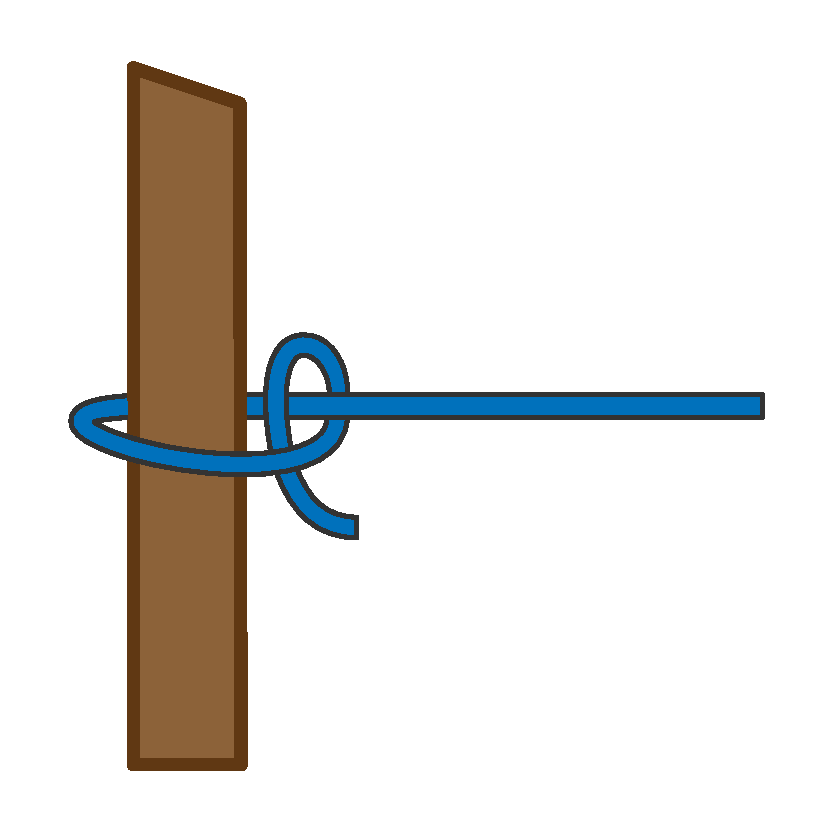
\includegraphics[width=0.8\textwidth]{Hoofdstukken/Schiemannen/pdf/halve_steek.pdf}
    \caption{Halve Steek}
    \label{pic:halve_steek}
  \end{minipage}
  \hfill
  \begin{minipage}[b]{0.32\textwidth}
    \centering
    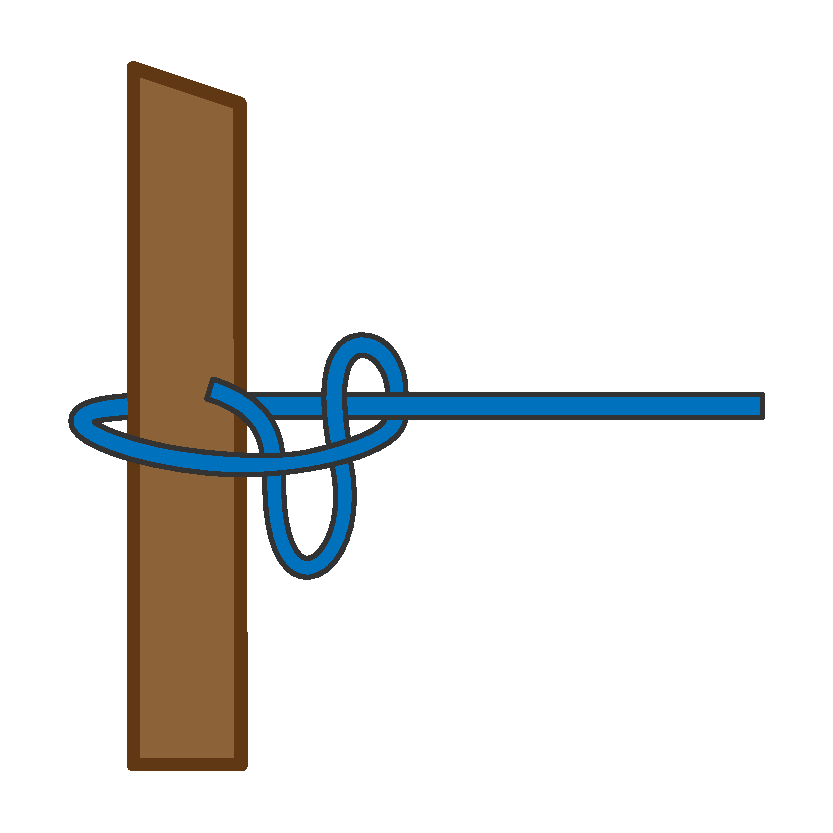
\includegraphics[width=0.8\textwidth]{Hoofdstukken/Schiemannen/pdf/slip_steek.pdf}
    \caption{Slipsteek}
    \label{pic:slip_steek}
    \end{minipage}
  \hfill
  \begin{minipage}[b]{0.32\textwidth}
    \centering
    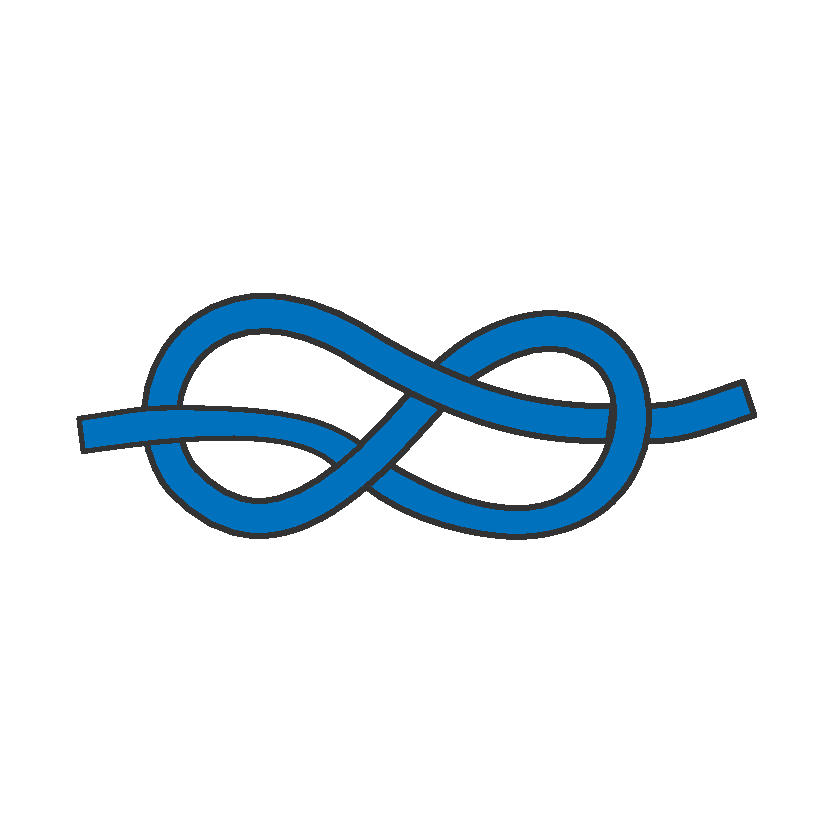
\includegraphics[width=0.8\textwidth]{Hoofdstukken/Schiemannen/pdf/achtknoop.pdf}
    \caption{Achtknoop}
    \label{pic:achtknoop}
  \end{minipage}
\end{figure}
\subsection{Platte knoop \hfill \textit{Figuur \ref{pic:platte_knoop}}}
Deze knoop is geschikt voor het verbinden van twee uiteinde van een touw van gelijke dikte. Deze knoop is niet geschikt voor situaties waar veel kracht op de lijn komt te staan. Hiervoor is een schootsteek beter geschikt.
\subsection{Schootsteek \hfill \textit{Figuur \ref{pic:schoot_steek}}}
Een schootsteek is geschikt om twee touwen van ongelijke dikte aan elkaar te maken. De knoop is ook geschikt voor touwen van gelijke dikte en kan veel kracht aan. Leg met het dikkere touw altijd de lus. Dat maakt de knoop makkelijker. 
\subsection{Mastworp \hfill \textit{Figuur \ref{pic:mastworp}}}
Deze knoop wordt veel gebruikt in pionieren en om je boot aan te leggen. De knoop trekt zichzelf strakker naar mate er meer kracht op komt. Daarnaast kun je een slipsteek op een mastworp leggen. Dit voorkomt dat de mastworp los kan schieten als er veel aan getrokken wordt. 
\begin{figure}[h]
  \centering
  \begin{minipage}[b]{0.32\textwidth}
  \centering
    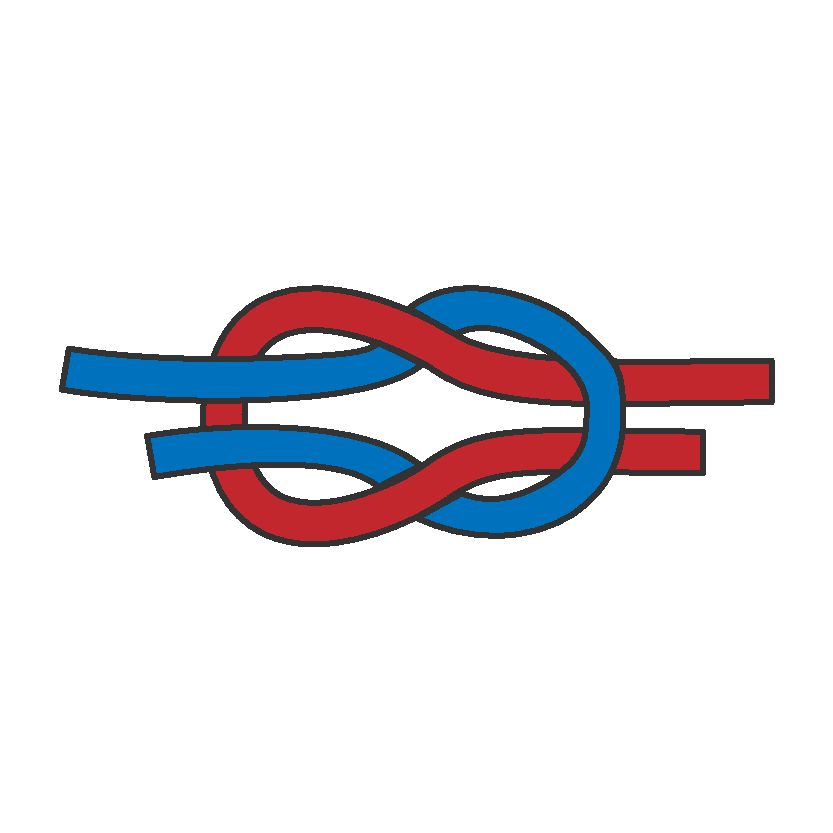
\includegraphics[width=0.8\textwidth]{Hoofdstukken/Schiemannen/pdf/platteknoop.pdf}
    \caption{Platte Knoop}
    \label{pic:platte_knoop}
  \end{minipage}
  \hfill
  \begin{minipage}[b]{0.32\textwidth}
    \centering
    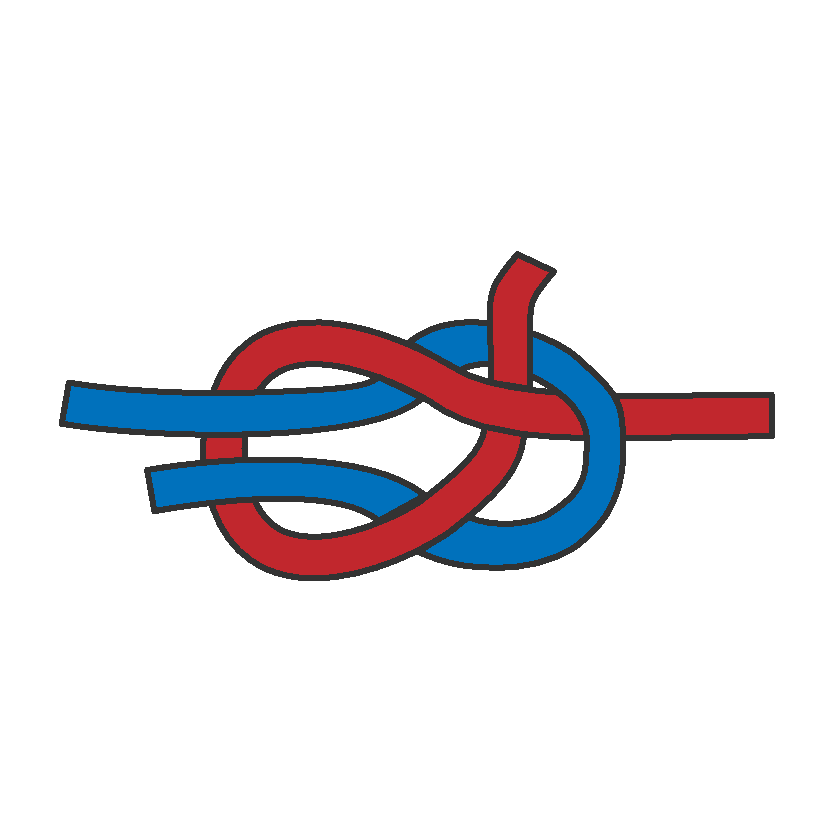
\includegraphics[width=0.8\textwidth]{Hoofdstukken/Schiemannen/pdf/schootsteek.pdf}
    \caption{Schootsteek}
    \label{pic:schoot_steek}
    \end{minipage}
  \hfill
  \begin{minipage}[b]{0.32\textwidth}
    \centering
    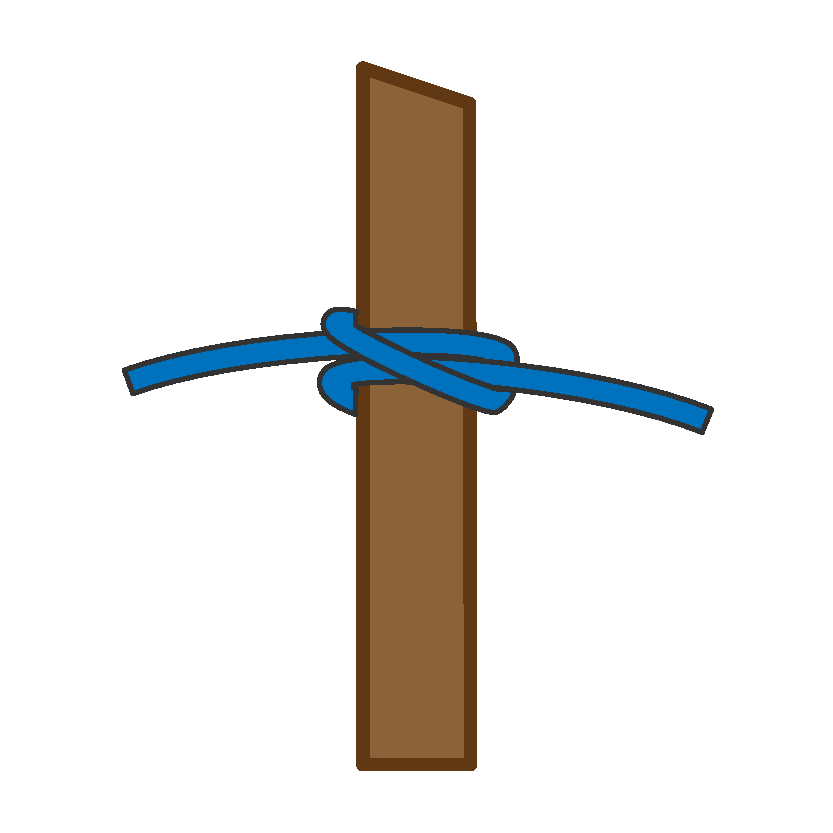
\includegraphics[width=0.8\textwidth]{Hoofdstukken/Schiemannen/pdf/mastworp.pdf}
    \caption{Mastworp}
    \label{pic:mastworp}
  \end{minipage}
\end{figure}
\subsection{Paalsteek \hfill \textit{Figuur \ref{pic:paal_steek}}} 
De paalsteek is bedoeld om een niet slippende lus in een touw te leggen. De lus is erg sterk, maar kan wel gemakkelijk weer losgehaald worden.
\subsection{Dubbele halve steek \hfill \textit{Figuur \ref{pic:dub_halve_steek}}}
Een dubbele halve steek is geschikt om lijnen strak aan een oog vast te maken. Dit is bijvoorbeeld handig als je aan wilt leggen met een meerpen. Je wikkelt eerst de lijn tweemaal om een oog en legt er vervolgens twee halve steken in. Dit maakt een mastworp. Je kan de eerste halve steek ook vervangen door een slipsteek.
\subsection{Een tros opschieten \hfill \textit{Figuur \ref{pic:opschieten}}}
Een tros opschieten is een manier om een lijn op te bergen zonder dat deze in de knoop raakt. Tijdens het opschieten maak je een aantal gelijke lussen. Aan het einde wikkel je de rest van het touw om de lussen en leg je een knoop als in het figuur. Opschieten staat ook wel bekend als opbossen.
\begin{figure}[h]
  \centering
  \begin{minipage}[b]{0.32\textwidth}
  \centering
    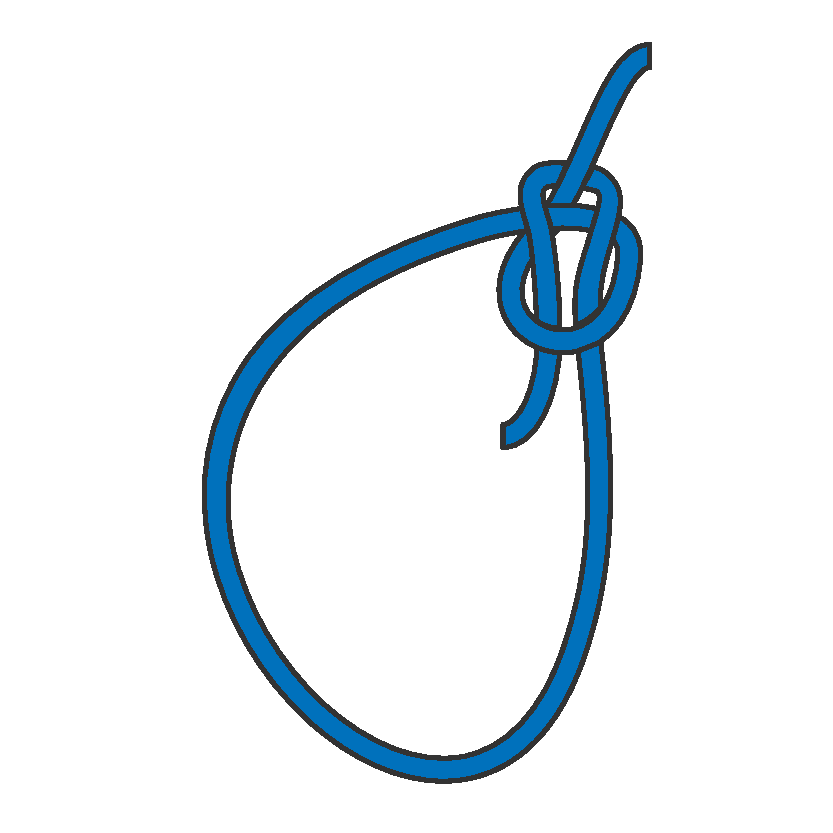
\includegraphics[width=\textwidth]{Hoofdstukken/Schiemannen/pdf/paalsteek.pdf}
    \caption{Paalsteek}
    \label{pic:paal_steek}
  \end{minipage}
  \hfill
  \begin{minipage}[b]{0.32\textwidth}
    \centering
    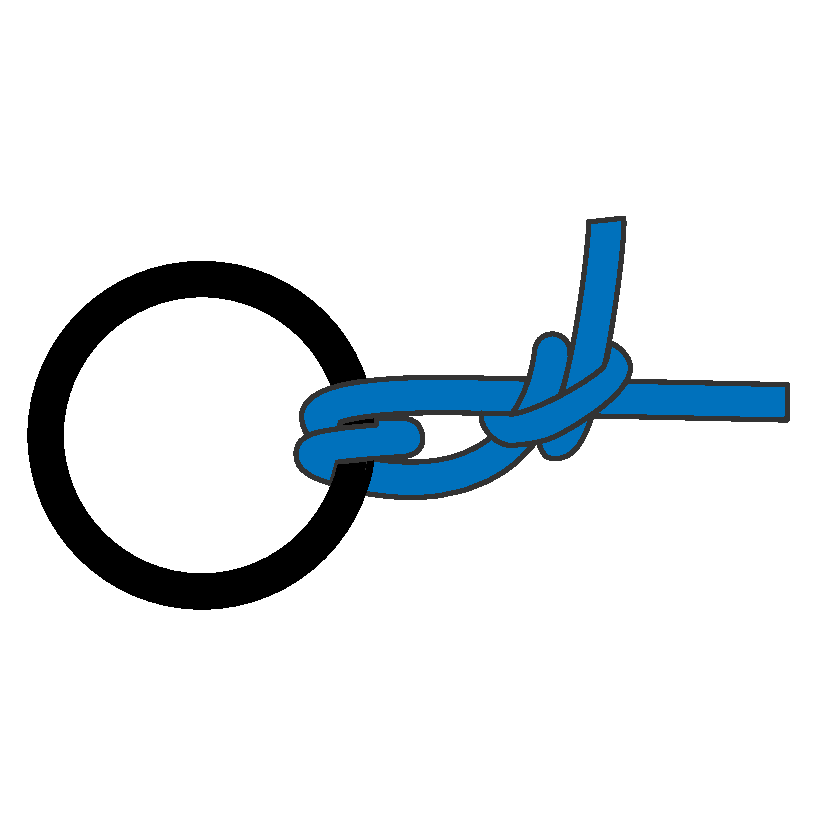
\includegraphics[width=\textwidth]{Hoofdstukken/Schiemannen/pdf/dubble_halve_steek.pdf}
    \caption{Dubbele halve steek}
    \label{pic:dub_halve_steek}
    \end{minipage}
  \hfill
   \begin{minipage}[b]{0.32\textwidth}
    \centering
    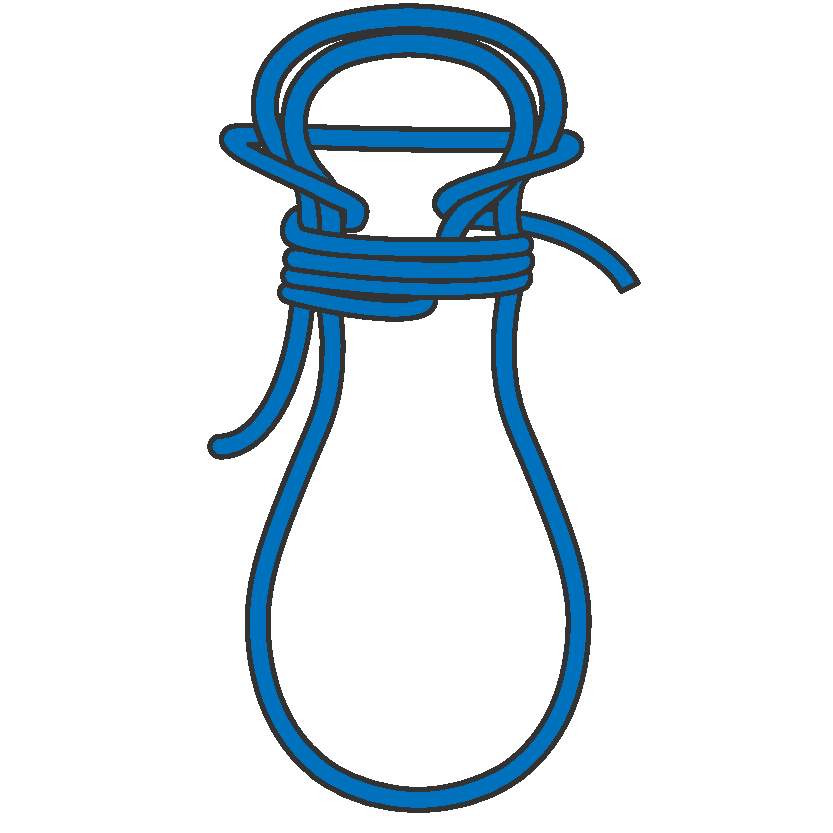
\includegraphics[width=\textwidth]{Hoofdstukken/Schiemannen/pdf/opbossen.pdf}
    \caption{Opschieten}
    \label{pic:opschieten}
    \end{minipage}
\end{figure}
\newpage
\subsection{Een kikker beleggen \hfill \textit{Figuur \ref{pic:kikker1}, \ref{pic:kikker2} \& \ref{pic:kikker3}}}
Wanneer je een kikker belegt, leg je een lijn vast op een kikker. Dit is nodig voor bijvoorbeeld het hijsen van het zeil. Belangrijk bij het beleggen van een kikker in een boot is dat je de ''eindlus'' aan de bovenzijde van de kikker legt. Anders kan deze er afvallen en de kikker losraken. Daarnaast moet je het lusje zo draaien dat het uiteinde weer in de richting van het vorige achtje gaat.
\begin{figure}[h]
  \centering
  \begin{minipage}[b]{0.32\textwidth}
  \centering
    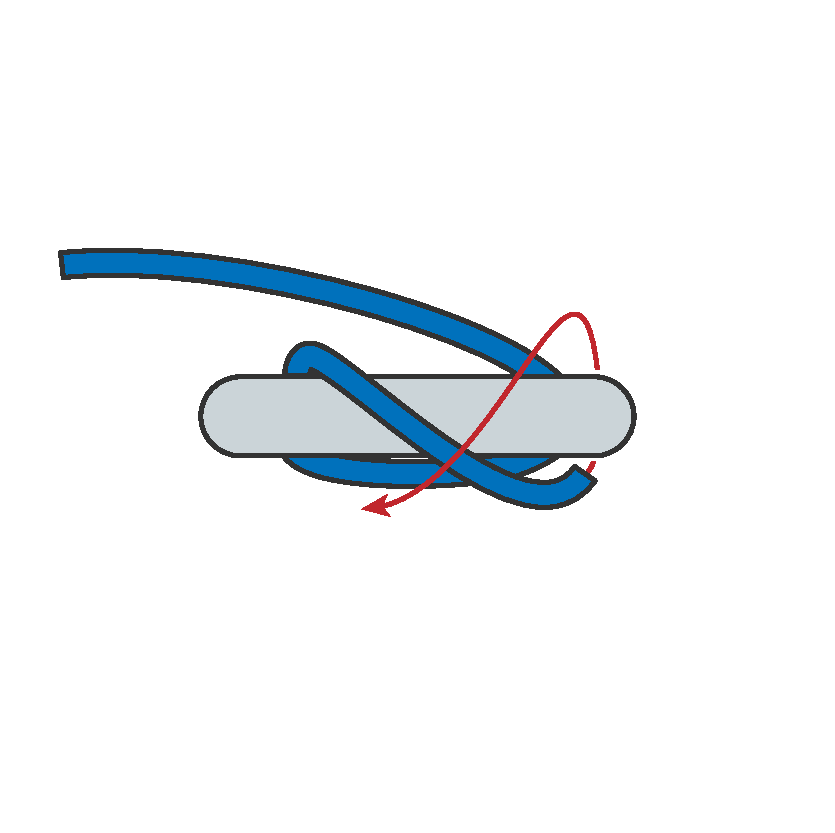
\includegraphics[width=\textwidth]{Hoofdstukken/Schiemannen/pdf/kikker1.pdf}
    \caption{Kikker 8'tjes}
    \label{pic:kikker1}
  \end{minipage}
  \hfill
  \begin{minipage}[b]{0.32\textwidth}
    \centering
    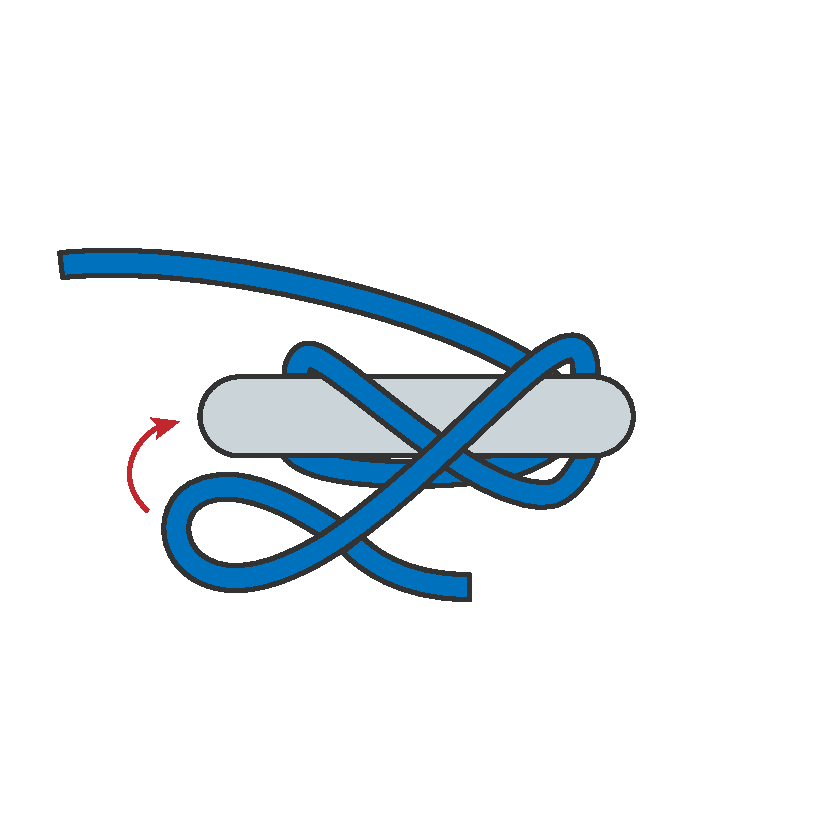
\includegraphics[width=\textwidth]{Hoofdstukken/Schiemannen/pdf/kikker2.pdf}
    \caption{Kikker eind lus}
    \label{pic:kikker2}
    \end{minipage}
  \hfill
   \begin{minipage}[b]{0.32\textwidth}
    \centering
    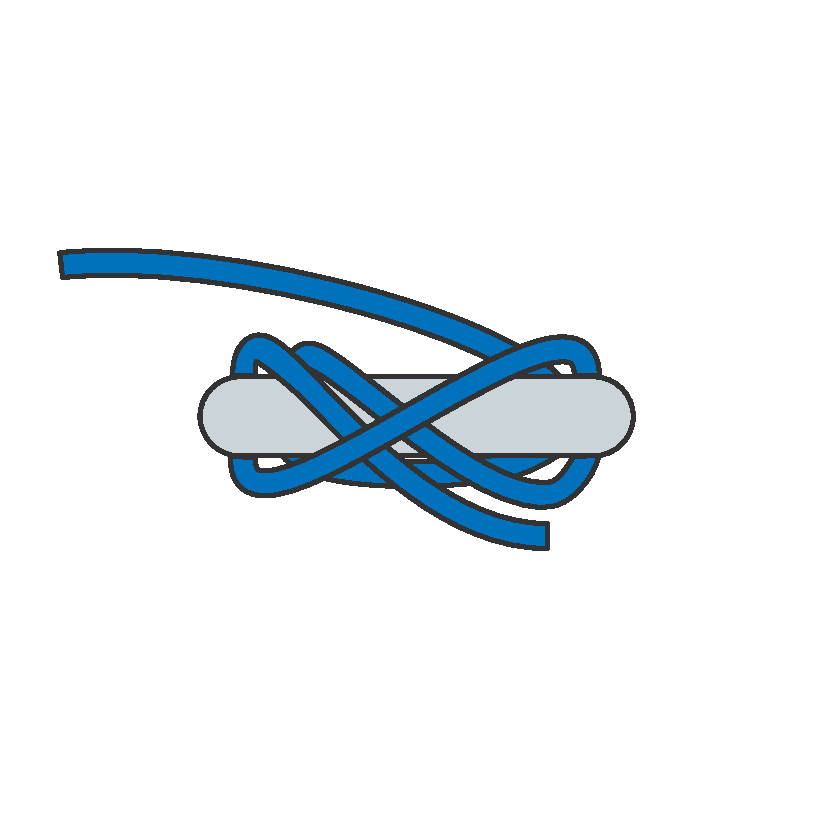
\includegraphics[width=\textwidth]{Hoofdstukken/Schiemannen/pdf/kikker3.pdf}
    \caption{Kikker afknopen}
    \label{pic:kikker3}
    \end{minipage}
\end{figure}
\section{Conclusie}
Na het lezen van dit hoofdstuk en het oefenen met de knopen, snap je het nut en toepassing van de verschillende knopen. Ook kan je alle knopen zonder voorbeeld leggen. Een instructeur heeft dit in de onderstaande tabel afgetekend.
\vspace{2cm}
\begin{table}[H]
\centering
\caption{Aftekenen knopen}
\label{my-label}
\begin{tabular}{|l|l|l|}
\hline
\textbf{Knoop of Handeling}  & \textbf{Paraaf} & \textbf{Paraaf} \\ \hline
\textit{Halve Steek}         &                 &                 \\ \hline
\textit{Slipsteek}          &                 &                 \\ \hline
\textit{Achtknoop}           &                 &                 \\ \hline
\textit{Platte Knoop}        &                 &                 \\ \hline
\textit{Schootsteek}        &                 &                 \\ \hline
\textit{Mastworp}            &                 &                 \\ \hline
\textit{Paalsteek}           &                 &                 \\ \hline
\textit{Dubbele halve steek} &                 &                 \\ \hline
\textit{Tros opschieten}     &                 &                 \\ \hline
\textit{Kikker beleggen}     &                 &                 \\ \hline
\end{tabular}
\end{table}